\chapter{Many fiber simulations} \label{chap:four}

	\begin{table}
		\rowcolors{1}{}{lightgray}
		\centering
		\caption{Reference parameters for all simulations presented in this chapter. Note that $n_j$ and $\delta_j$ are functions of $j$. For each $j$, $n_j$ is constant and $\delta_j$ is linear. \label{table:manyfiber_reference}}
		\begin{tabular}{lcrclcr}
			$m$ & = & 10 & \hspace{1in} & $\ell_-$ & = & 1 \\
			$n_j$ & = & 96 & & $\ell_+$ & = & 1 \\
			$n_+$ & = & 360 & & $\ell$ & = & 1 \\
			$n_-$ & = & 310 & & $\gamma$ & = & 100 \\
			$x^{(-)}$ & = & -110 & & $\beta$ & = & 10 \\
			$y^{(-)}$ & = & 0 & & $\eps_-$ & = & 0.1 \\
			$x^{(+)}$ & = & -160 & & $\eps_+$ & = & 1 \\
			$y^{(+)}$ & = & 110 & & $\eps$ & = & 0.1 \\
			$\delta_j$ & = & 10$j$ & & $\sigma$ & = & 1
		\end{tabular}
	\end{table}

	In Chapter~\ref{chap:three} we discussed three different simulation experiments: a fiber standing free of load, a fiber under compression from the top substrate, and the top substrate detaching from the fiber. Here we look at the compression experiment with ten fibers. As before we have a set of reference parameters (see Table~\ref{table:manyfiber_reference}). We run the compression experiment for the reference parameters and three variations of the parameters, specifically varying $\beta$, $\gamma$, and $\eps_+$.

	\begin{figure}
		\begin{center}
			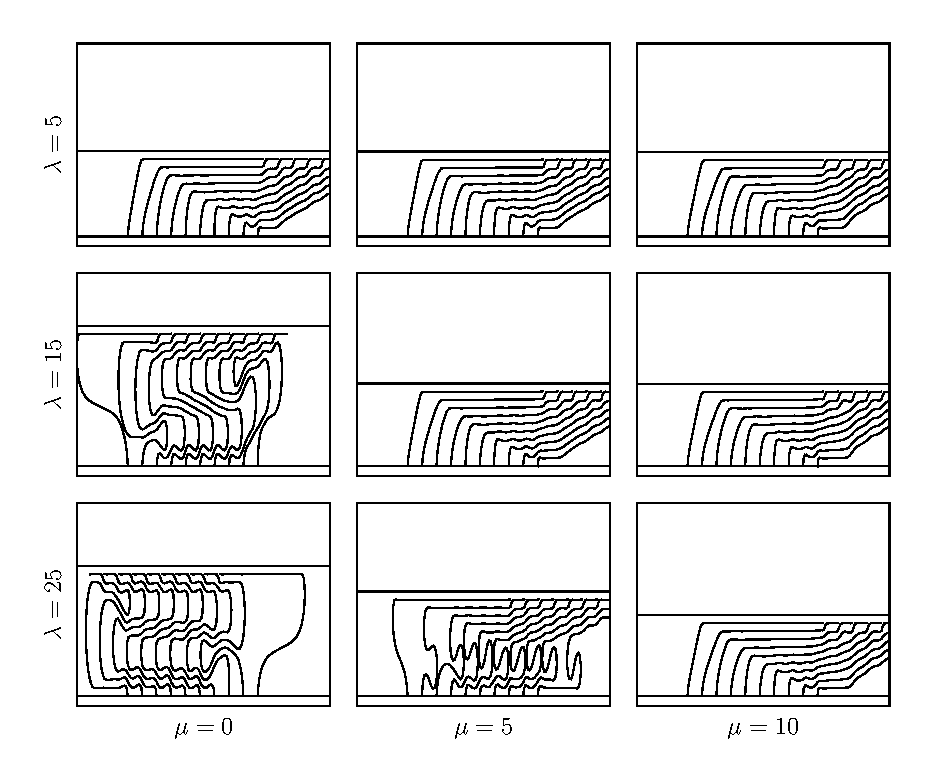
\includegraphics[scale=1]{./fig/ch4/grid.eps}
		\end{center}		
		\caption{Equilibrium configurations of ten fibers with 96 particles each for varying loads. The top left plot is a configuration with a load of $\lambda = 5$ and $\mu = 0$. The configurations to the right and below correspond to an increasing $\mu$ and increasing $\lambda$ respectively. All configurations use the reference parameters in Table~\ref{table:manyfiber_reference}.
		\label{fig:grid}}
	\end{figure}
	
	We consider nine simulations with values of $\lambda = 5, 15, 25$ and $\mu = 0, 5, 10$. In Figure~\ref{fig:grid} we see a high level view of each simulation for the reference parameters. Keeping the horizontal component of the load zero, we see an increase in curvature of all ten fibers as we increase $\lambda$. One explanation for this is that the torsional and extensible springs don't have enough time to slide along the top substrate and align to it. As the magnitude of the vertical component of the load is increased the fibers become more likely to buckle. 
	
	If we increase the horizontal component of the load the story changes. We are able to maintain the aligned compressed configuration for larger magnitudes of the load if the horizontal component is sufficiently large. It would seem that the ratio between vertical and horizontal component for the reference parameters is the deciding factor for whether or not fibers will buckle.

	\begin{figure}
		\begin{center}
			\includegraphics[scale=1]{./fig/ch4/grid_b100.eps}
		\end{center}		
		\caption{Equilibrium configurations of varying loads. All configurations are directly comparable to Figure~\ref{fig:grid} with the exception that $\beta = 100$.
		\label{fig:grid_b100}}
	\end{figure}

	In Figure~\ref{fig:grid_b100} we increase $\beta$ to one hundred. This is an order of magnitude increase from the reference parameters and it prevents buckling at all selected loads. Qualitatively there is no discernible difference in any of the nine simulations with the one exception that the fibers buckle to the left with no horizontal component of the load. This bias for the load with no horizontal component could be caused by a numerical artifact or an asymmetry in the number of atoms on the top substrate to the left of the leftmost fiber versus to the right of the rightmost fiber. Regardless of the reason, the configuration when $\mu = 0$ appears close to a mirror image of configurations for $\mu > 0$.
	
	\begin{figure}
		\begin{center}
			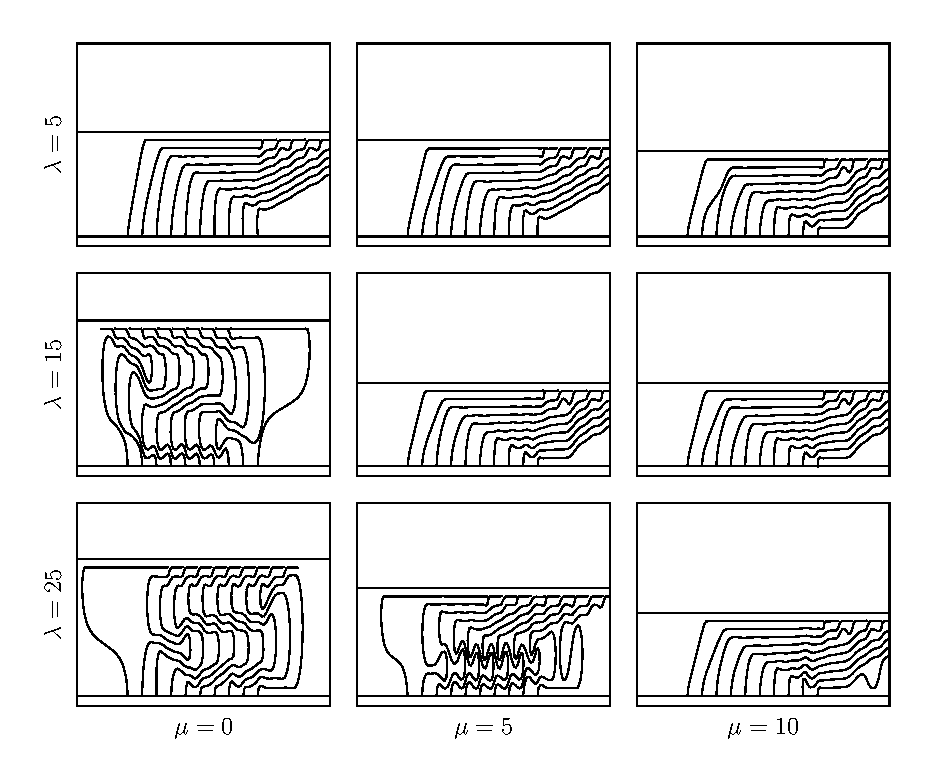
\includegraphics[scale=1]{./fig/ch4/grid_g1000.eps}
		\end{center}		
		\caption{Equilibrium configurations of varying loads. All configurations are directly comparable to Figure~\ref{fig:grid} with the exception that $\gamma = 1000$.
		\label{fig:grid_g1000}}
	\end{figure}
	
	We observe that the increase in the torsional spring strength prevents buckling to happen anywhere except the junction between the fiber and the substrate. On the other hand when we increase the extensible spring constant by an order of magnitude the buckling patterns are the same as those observed for the reference parameters. Comparing Figure~\ref{fig:grid_g1000} to Figure~\ref{fig:grid}, the same sets of configurations are present in both. With $\gamma$ sufficiently large and vdW sufficiently weak, further increasing $\gamma$ plays a negligible role because the distance between particles on a fiber is already close to $\ell$. This confirms are choice for $\gamma$ in the reference parameters maintains extensional rigidity.
	
	\begin{figure}
		\begin{center}
			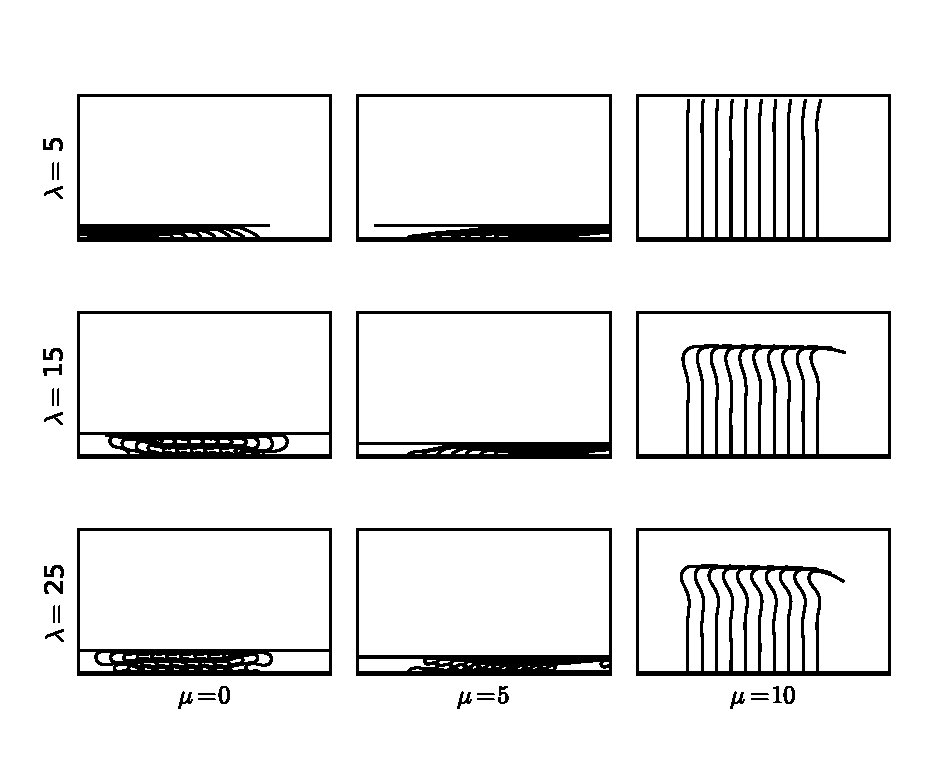
\includegraphics[scale=1]{./fig/ch4/grid_et0.1.eps}
		\end{center}		
		\caption{Equilibrium configurations of varying loads. All configurations are directly comparable to Figure~\ref{fig:grid} with the exception that $\eps_+ = 0.1$.
		\label{fig:grid_et0.1}}
	\end{figure}

	Next, consider the situation when all vdW strengths in the system are the same. In Figure~\ref{fig:grid_et0.1} we reduce $\eps_+$ to 0.1 and present the results for nine different loads while keeping the rest of the parameters equal to the reference values. For $\mu = 0$ or $5$ the configurations are comparable. We further observe that the horizontal component of the load can be strong enough to cause the top substrate to slide off the fibers overpowering the vdW interaction. This happens for all values of the vertical component of the load that we have considered.
	
	We perform the detachment experiment on a configuration of many fibers versus one fiber in order to determine how the model scales in computational expense. However, computationally the model can be improved to obtain a better computational scaling with more particles. Ideally this model is so simple \textit{because} you want to explore very large systems under the assumption the model will be approximately correct or insightful in some way.

TODO (last paragraph is a mess) + physical and time scale
TODO (table of computation times)

	